% MacStarStacker 使い方ガイド
% ビルド: docs/manual/build.sh（LuaLaTeX）。
% スクリーンショットは DocumentationScreenshotTests（MacStarStacker.swiftpm/Tests）で撮る。手順は README.md を参照
\documentclass[paper=a4paper,fontsize=11pt,jafontsize=10.5pt,line_length=42zw,number_of_lines=42,
  head_space=20mm,foot_space=14mm]{jlreq}
\usepackage{manual-style}

\begin{document}

% 表紙
\thispagestyle{empty}
\begin{tikzpicture}[remember picture,overlay]
  \fill[black!92] (current page.north west) rectangle (current page.south east);
  \node[anchor=north,inner sep=0pt] at ($(current page.north)+(0,-2.2cm)$)
    {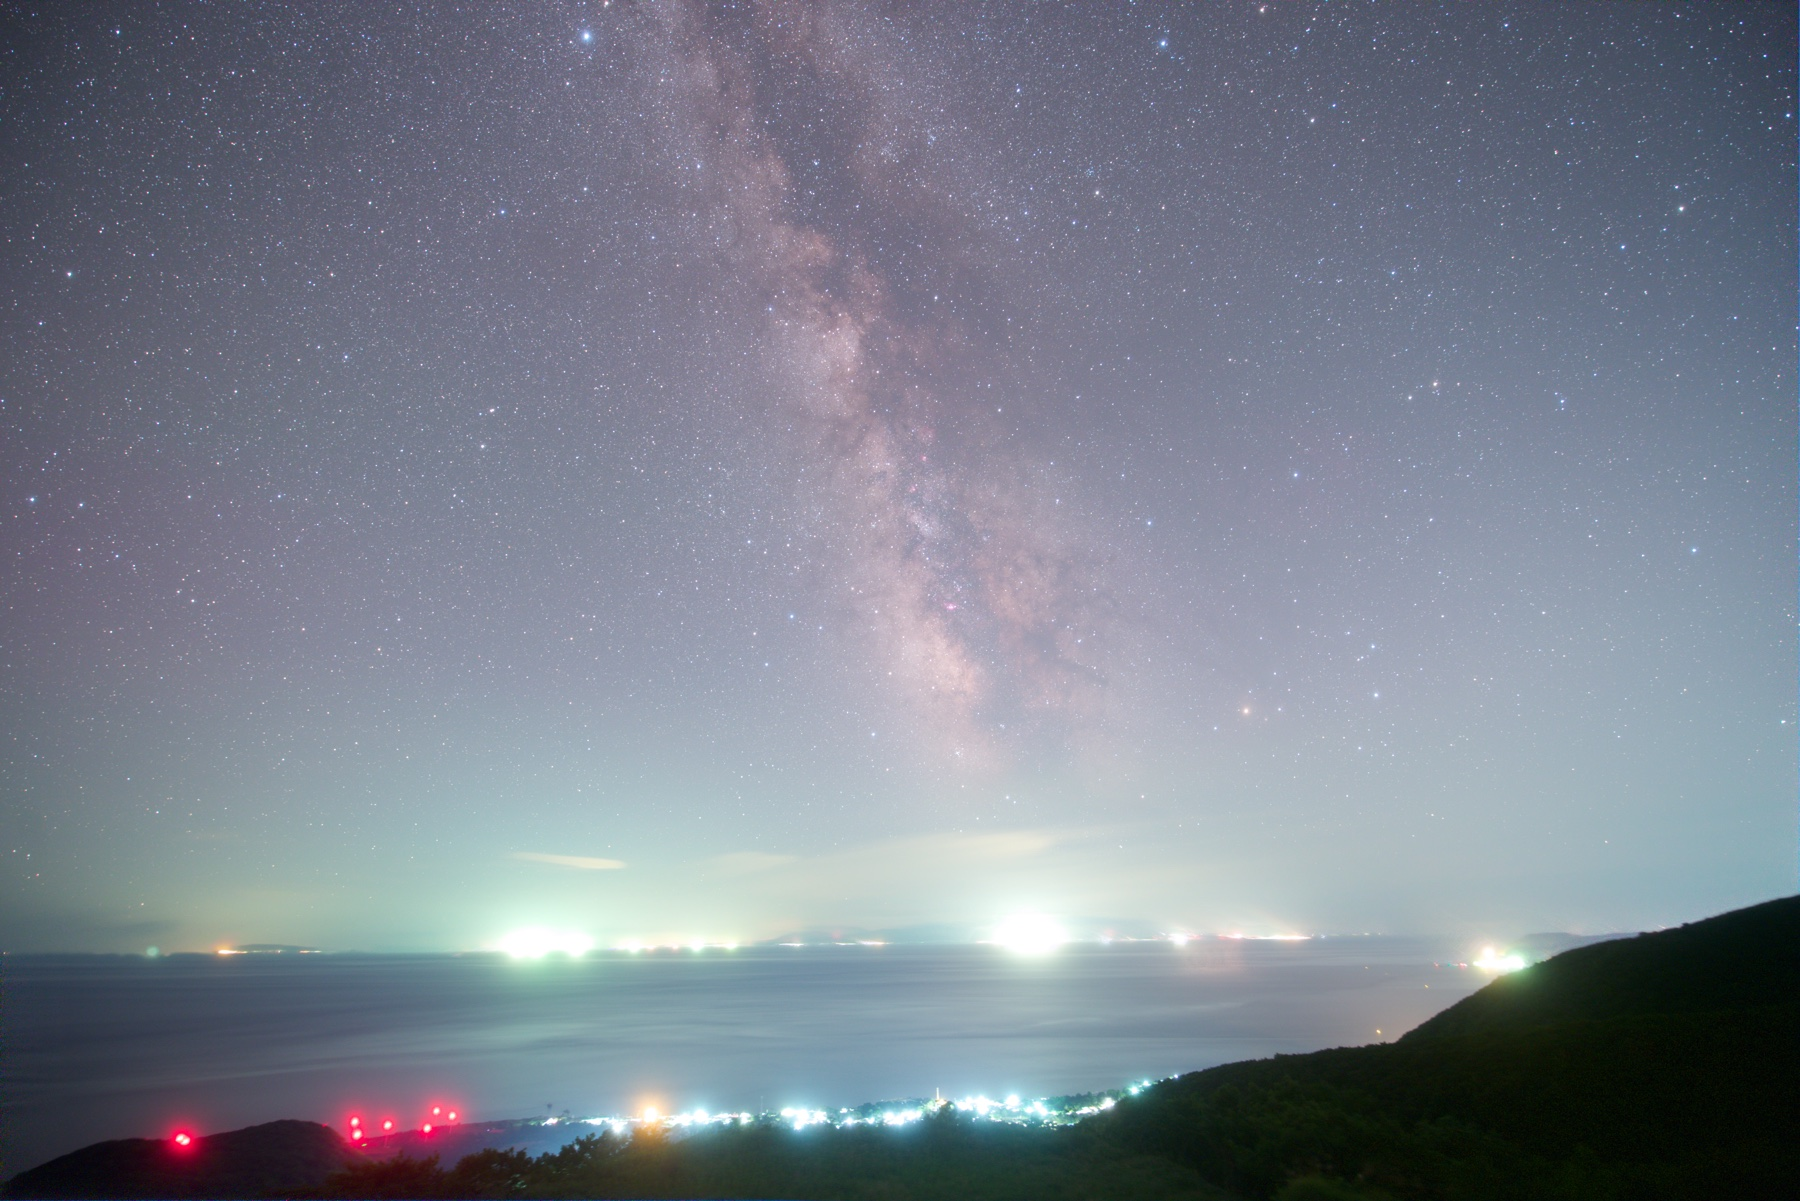
\includegraphics[width=0.86\paperwidth]{figures/photo_nightscape}};
  \node[anchor=north,text=white,font=\sffamily\bfseries\fontsize{30}{36}\selectfont]
    at ($(current page.north)+(0,-15.8cm)$) {MacStarStacker};
  \node[anchor=north,text=accent,font=\sffamily\bfseries\fontsize{20}{26}\selectfont]
    at ($(current page.north)+(0,-17.6cm)$) {使い方ガイド};
  \node[anchor=north,text=white!80,font=\sffamily\large,align=center]
    at ($(current page.north)+(0,-19.6cm)$) {星景写真のスタッキング（合成）アプリ\\[0.6ex]
      はじめての方でも、画面を見ながら順番に進められるように説明します};
  \node[anchor=south,text=white!70,font=\sffamily,align=center]
    at ($(current page.south)+(0,2.4cm)$) {バージョン 2.0\\[0.4ex]\small https://github.com/Geology-cat/MacStarStacker};
  \node[anchor=south east,text=white!55,font=\sffamily\scriptsize]
    at ($(current page.south east)+(-1.2cm,0.8cm)$) {表紙の写真：MacStarStacker の新星景モードで合成した例};
\end{tikzpicture}
\null
\clearpage

\tableofcontents
\clearpage

\section{はじめに}

\subsection{MacStarStacker でできること}

MacStarStacker は、星空を何枚も続けて撮った写真を1枚に重ね合わせる（\textbf{スタッキング}する）アプリです。
重ね合わせると、1枚だけでは目立つざらざらしたノイズが減り、淡い天の川までなめらかに写ります。

\begin{itemize}[itemsep=0.4ex]
  \item \textbf{ノイズを減らす}：同じ星空の写真を平均して、ノイズの少ない1枚にします（平均・中央値）。
  \item \textbf{星と地上を両方くっきり}：空は星に、地上は地上に合わせてそれぞれ重ね、1枚にまとめます（新星景モード）。
  \item \textbf{星の軌跡を描く}：星が動いた跡を線として残します。飛行機や人工衛星の光は取り除けます（比較明合成）。
  \item \textbf{RAW のまま合成}：カメラの RAW ファイルを現像せずに合成し、Lightroom などで元の RAW と同じように調整できる DNG で書き出せます。
  \item \textbf{タイムラプス動画}：読み込んだ写真をつないで動画（MP4）にします。
\end{itemize}

\begin{figure}[H]
\centering
\begin{minipage}[t]{0.485\linewidth}\centering
  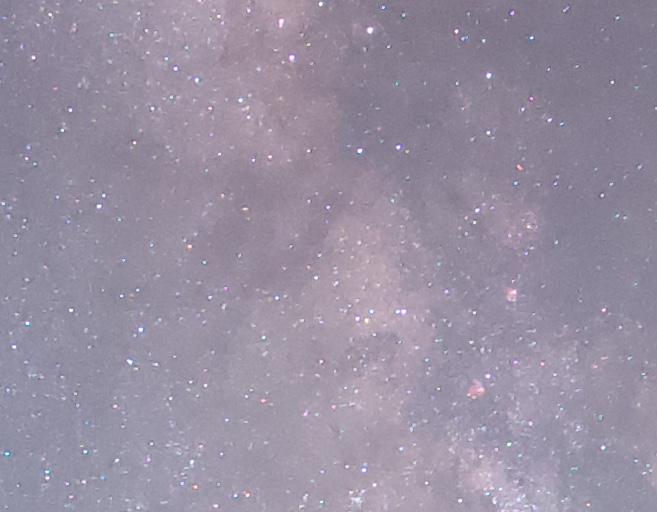
\includegraphics[width=\linewidth]{figures/photo_single_crop}\\[0.3ex]
  {\small 1枚だけの写真（一部を拡大）}
\end{minipage}\hfill
\begin{minipage}[t]{0.485\linewidth}\centering
  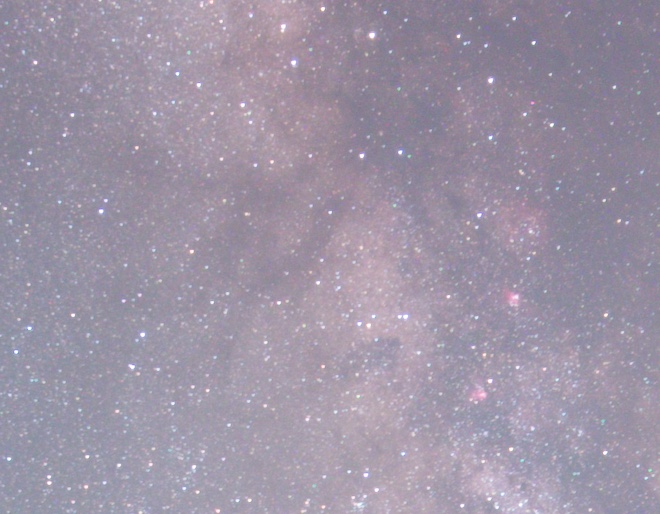
\includegraphics[width=\linewidth]{figures/photo_stacked_crop}\\[0.3ex]
  {\small 25枚をスタッキングした結果（同じ所）}
\end{minipage}
\caption{スタッキングするとノイズが減り、星と天の川がなめらかになります}
\end{figure}

\subsection{はじめに知っておきたい言葉}

このガイドでは、次の言葉を使います。

\begin{center}
\small
\begin{tabularx}{\linewidth}{>{\bfseries}l X}
\toprule
言葉 & 意味 \\
\midrule
スタッキング（合成） & 何枚もの写真を重ね合わせて1枚にすること。 \\
Light（ライト） & 星空を撮った、合成したい写真そのもの。 \\
Dark（ダーク） & レンズにキャップをして、Light と同じ設定（露出時間・ISO・温度）で撮った真っ暗な写真。センサーのむらや熱によるノイズを差し引くのに使います（なくてもかまいません）。 \\
Flat（フラット） & 明るさが均一な面（白い布や夜明け前の空など）を撮った写真。周辺が暗くなる「周辺減光」やごみの影を補正します（なくてもかまいません）。 \\
Bias（バイアス） & キャップをして、いちばん短い露出時間で撮った写真。センサーの基準の明るさを差し引きます（なくてもかまいません）。 \\
基準画像 & 位置を合わせるときの「お手本」にする1枚。ファイルリストの\ui{★}で選びます。 \\
アライメント & 写真ごとの星の位置のずれを合わせること（位置合わせ）。 \\
RAW / DNG & カメラが記録する、現像前のデータ（CR2・NEF・ARW など）。DNG は Adobe が決めた RAW の形式です。 \\
新星景 & 星空と地上の風景を1枚に収めた写真。星に合わせると地上が、地上に合わせると星がぶれるので、空と地上を分けて合成します。 \\
比較明合成 & 写真を重ねるとき、画素ごとにいちばん明るい値を残す合成。星の軌跡（スタートレイル）になります。 \\
\bottomrule
\end{tabularx}
\end{center}

\subsection{動作環境}\label{sec:requirements}

MacStarStacker には、動かす Mac に合わせた2つの版があります。どちらも同じ機能が使えます。

\begin{center}
\small
\begin{tabularx}{\linewidth}{l X}
\toprule
版（DMG の名前） & 動く Mac \\
\midrule
\textsf{macOS14-Universal} & macOS 14 (Sonoma) 以降の Mac（Apple シリコン・Intel のどちらも） \\
\textsf{macOS10.13-Universal} & Intel の Mac は macOS 10.13 (High Sierra) 以降、Apple シリコンの Mac は macOS 11 以降 \\
\bottomrule
\end{tabularx}
\end{center}

\begin{memo}[どちらを選べばいい？]
macOS 14 以降の Mac では \textsf{macOS14} 版を使ってください。それより古い macOS の Mac では \textsf{macOS10.13} 版を使います。
\end{memo}

読み込める写真は次のとおりです。
\begin{itemize}[itemsep=0.2ex]
  \item RAW：Canon（CR2・CR3）、Nikon（NEF）、Sony（ARW）、Fujifilm（RAF）、OM System / Olympus（ORF）、Panasonic（RW2）、Pentax（PEF）、DNG
  \item そのほか：TIFF、FITS、JPEG、PNG、HEIC
\end{itemize}

\begin{hint}[メモリの目安]
中央値合成やシグマクリッピング、新星景モードは、全部の写真のデータを一度にメモリに置くため、たくさんのメモリを使います。
2000万画素の RAW を20〜30枚なら、16GB 以上のメモリがあると安心です。足りないときは、始める前にメッセージでお知らせします。
\end{hint}

\clearpage
\section{インストール}

\subsection{DMG をダウンロードして開く}

\begin{steps}
  \item GitHub のリリースのページ（\url{https://github.com/Geology-cat/MacStarStacker/releases}）から、お使いの Mac に合った DMG ファイルをダウンロードします（どちらを選ぶかは\pageref{sec:requirements}ページの「動作環境」を見てください）。
  \item ダウンロードした DMG ファイルをダブルクリックします。次のようなウインドウが開きます。
\end{steps}

\begin{figure}[H]
\centering
\installshot{install_dmg}{0.9\linewidth}{
  \labelat{app}{-90}{1.3}{アプリ本体}
  \labelat{guide}{-90}{1.5}{このガイド}
  \labelat{installer}{-90}{1.3}{かんたんインストーラ}
  \labelat{readme}{-90}{1.4}{はじめに読む説明}
}
\caption{DMG を開いたところ}
\end{figure}

\subsection{かんたんインストーラでインストールする（おすすめ）}

「かんたんインストーラ」は、次の3つをまとめて行います。
\begin{enumerate}[label=(\arabic*),itemsep=0.2ex]
  \item MacStarStacker を「アプリケーション」フォルダへコピーする
  \item 初回起動の確認（Gatekeeper）を解除する
  \item MacStarStacker を起動する
\end{enumerate}

\begin{steps}
  \item DMG の中の\ui{かんたんインストーラ.scpt}をダブルクリックします。「スクリプトエディタ」が開きます。
  \item ウインドウの上にある\ui{▶}（実行）ボタンを押します。
\end{steps}

\begin{figure}[H]
\centering
\installshot{install_script}{0.8\linewidth}{
  \markbox{run}
  \callout{1}{run}{-150}{1.8}
}
\caption{スクリプトエディタで開いたところ。\num{1}の ▶（実行）を押します}
\end{figure}

\begin{steps}[resume]
  \item 確認のメッセージが出たら\ui{インストール}を押します。
\end{steps}

\begin{figure}[H]
\centering
\installshot{install_dialog}{0.55\linewidth}{
  \markbox{install}
  \callout{1}{install}{-60}{1.3}
}
\caption{インストールの確認。\num{1}の\ui{インストール}を押します}
\end{figure}

\begin{steps}[resume]
  \item 「アプリケーション」フォルダに書き込むのに管理者の許可が必要なときは、パスワードを聞かれます。Mac にログインするときのパスワードを入れてください。
  \item しばらくすると MacStarStacker が起動し、「インストールが終わり、MacStarStacker を起動しました。」と表示されます。これで完了です。DMG は取り出してかまいません（Finder のサイドバーの「MacStarStacker」の横にある取り出しボタンを押します）。
\end{steps}

\begin{memo}[新しい版に入れ替えるとき]
すでに MacStarStacker が入っていても、同じ手順でかまいません。古いものを終了させてから、新しいものに置き換えます。
\end{memo}

\subsection{手動でインストールする}\label{sec:install-manual}

かんたんインストーラを使わない場合は、次のようにします。

\begin{steps}
  \item DMG のウインドウで、\ui{MacStarStacker.app}を\ui{Applications}のフォルダへドラッグします。
  \item 「アプリケーション」フォルダの MacStarStacker を開きます。
\end{steps}

MacStarStacker は Apple の Developer ID による署名・公証をしていないため、初めて開くときに macOS が確認のメッセージを出し、そのままでは開けません。次の手順で開いてください（2回目からはふつうに開けます）。

\paragraph{macOS 15 (Sequoia) 以降}
\begin{steps}
  \item 「“MacStarStacker.app”は開いていません」というメッセージが出たら、\ui{完了}を押して閉じます（\ui{ゴミ箱に入れる}は押さないでください）。
  \item アップルメニュー \menu{→ システム設定 → プライバシーとセキュリティ}を開きます。
  \item 下の方の「セキュリティ」の欄に「“MacStarStacker”は…ブロックされました」と出ているので、\ui{このまま開く}を押します。
  \item パスワードを入れ、もう一度出るメッセージで\ui{開く}を押します。
\end{steps}

\begin{figure}[H]
\centering
\installshot{install_blocked}{0.34\linewidth}{
  \markbox{done}
  \callout{1}{done}{-90}{1.2}
}
\caption{初めて開いたときのメッセージ（macOS 15）。\num{1}の\ui{完了}を押して閉じます}
\end{figure}

\begin{figure}[H]
\centering
\installshot{install_gatekeeper}{0.75\linewidth}{
  \markbox{openanyway}
  \calloutright{1}{openanyway}
}
\caption{システム設定の「プライバシーとセキュリティ」の下の方。\num{1}の\ui{このまま開く}を押します}
\end{figure}

\paragraph{macOS 14 (Sonoma) 以前}
\begin{steps}
  \item 「アプリケーション」フォルダの MacStarStacker を、\key{control}キーを押しながらクリック（または右クリック）します。
  \item 出てきたメニューから\ui{開く}を選び、メッセージでもう一度\ui{開く}を押します。
\end{steps}

\subsection{アンインストール（削除）}

「アプリケーション」フォルダの MacStarStacker をゴミ箱に入れるだけです（ウインドウの位置などの小さな設定が残るだけで、ほかに消すものはありません）。

\clearpage
\section{画面の見方}\label{sec:screen}

MacStarStacker を起動すると、次のような画面が開きます。画面は左・中央・右の3つに分かれています。

\begin{figure}[H]
\centering
\begin{screenshot}{main_loaded}
  \calloutabove{1}{filelist}
  \calloutabove{2}{canvas}
  \calloutabove{3}{settings}
  \calloutleft{4}{base}
  \calloutleft{5}{star}
  \markbox{start}
  \calloutright{6}{start}
\end{screenshot}
\caption{MacStarStacker の画面（写真を読み込んだところ）}
\end{figure}

\begin{callouts}
\co{1} \textbf{ファイルリスト}：読み込んだ写真の一覧です。Light・Dark・Flat・Bias の種類ごとに分かれています（\ref{sec:filelist}節）。
\co{2} \textbf{プレビュー}：選んだ写真や、合成した結果を大きく表示します。新星景モードでは、ここで空と地上をブラシで塗り分けます（\ref{sec:preview}節）。
\co{3} \textbf{設定}：合成のしかた、書き出す形式などを選びます。上のタブで\ui{スタック}と\ui{タイムラプス}を切り替えます（\ref{sec:stacking}節）。
\co{4} \textbf{基準画像}：いま基準になっている写真の名前と、撮影の情報（レンズ・焦点距離・F値・ISO・露出時間）です。
\co{5} \ui{★}：押した写真が基準画像になります。黄色の★が基準画像です。
\co{6} \ui{★ スタッキング開始}：合成を始めます。
\end{callouts}

\subsection{メニューとキーボードショートカット}

よく使う操作は、メニューやキーボードからも行えます。

\begin{center}
\small
\begin{tabularx}{\linewidth}{l l X}
\toprule
メニュー & キー & はたらき \\
\midrule
ファイル → Light 画像を追加… & \key{⌘}\,\key{O} & Light の写真を選んで読み込みます。 \\
ファイル → スタック結果を書き出す… & \key{⌘}\,\key{S} & 合成した結果をファイルに保存します。 \\
編集 → 取り消す & \key{⌘}\,\key{Z} & 写真の追加・削除を1つ前に戻します。 \\
編集 → マスクをクリア & \key{⌘}\,\key{K} & ブラシで塗ったマスクを消します。 \\
編集 → すべてクリア… & & 写真・結果・マスク・設定をすべて消して、起動した直後に戻します。 \\
処理 → スタッキング開始 & \key{⌘}\,\key{R} & 合成を始めます。 \\
MacStarStacker → 終了 & \key{⌘}\,\key{Q} & アプリを終了します。 \\
\bottomrule
\end{tabularx}
\end{center}

\clearpage
\section{まずはやってみよう（5つの手順）}\label{sec:quickstart}

まずは、いちばん基本の「平均」でノイズの少ない1枚を作ってみましょう。
同じ構図で続けて撮った星空の写真（10〜30枚くらい）を用意してください。

\begin{center}
\begin{tikzpicture}[node distance=0.35cm,
  box/.style={draw=accentdark,fill=accent!12,rounded corners=3pt,minimum height=1.1cm,text width=2.35cm,
    align=center,font=\sffamily\small},
  arr/.style={-{Stealth[length=2.4mm]},accentdark,line width=1pt}]
  \node[box] (a) {\textbf{1} 写真を\\読み込む};
  \node[box,right=of a] (b) {\textbf{2} 基準画像を\\選ぶ};
  \node[box,right=of b] (c) {\textbf{3} 合成のしかたを\\選ぶ};
  \node[box,right=of c] (d) {\textbf{4} スタッキング\\開始};
  \node[box,right=of d] (e) {\textbf{5} 結果を\\書き出す};
  \draw[arr] (a) -- (b); \draw[arr] (b) -- (c); \draw[arr] (c) -- (d); \draw[arr] (d) -- (e);
\end{tikzpicture}
\end{center}

\subsection*{手順1　写真を読み込む}

\begin{figure}[H]
\centering
\begin{screenshot}{main_empty}
  \markbox{add}
  \calloutleft{1}{add}
\end{screenshot}
\caption{起動した直後の画面}
\end{figure}

\begin{steps}
  \item ファイルリストの\ui{＋ 追加}を押し、合成したい写真（Light）を選びます。\key{⌘}キーや\key{shift}キーを押しながらクリックすると、何枚もまとめて選べます。フォルダを選ぶと、中の写真をまとめて読み込みます。
  \item または、Finder から写真（またはフォルダ）をファイルリストにドラッグ＆ドロップしても読み込めます。
\end{steps}

読み込むと、ファイルリストに写真の名前が並び、プレビューに1枚目が表示されます。

\subsection*{手順2　基準画像を選ぶ}

最初に読み込んだ写真が、自動で基準画像（黄色の\ui{★}）になります。ほかの写真にしたいときは、その写真の\ui{☆}を押します。
ふつうは真ん中あたりの写真を選ぶと、全体のずれが小さくなります。

\subsection*{手順3　合成のしかたを選ぶ}

右の設定の\ui{スタック方式}で\ui{平均 (Average)}を選び、\ui{アライメント（星の位置合わせ）}にチェックが入っていることを確かめます（最初からこの設定になっています）。

\subsection*{手順4　スタッキング開始}

\ui{★ スタッキング開始}を押します（\key{⌘}\,\key{R}でも始まります）。プレビューの下に進み具合が表示されます。

\begin{figure}[H]
\centering
\begin{screenshot}{main_stacking}
  \markbox{progress}
  \calloutbelow{1}{progress}
\end{screenshot}
\caption{合成しているところ。\num{1}に進み具合が表示されます}
\end{figure}

\subsection*{手順5　結果を書き出す}

合成が終わると、プレビューに結果が表示されます。\ui{書き出し \& 実行}の上の欄で形式を選び、\ui{結果を書き出す…}を押して保存します（\ref{sec:export}節）。
迷ったら、まずは\ui{RAW (DNG)}で保存しておくと、あとで Lightroom などで明るさや色を自由に調整できます。

\begin{figure}[H]
\centering
\begin{screenshot}{main_result_average}
  \calloutabove{1}{toggle}
  \calloutright[0.3]{3}{format}
  \calloutright[-0.2]{2}{status}
  \markbox{export}
  \calloutright{4}{export}
\end{screenshot}
\caption{合成が終わったところ}
\end{figure}

\begin{callouts}
\co{1} \ui{元画像を表示}／\ui{スタック結果を表示}：合成前の写真と結果を切り替えて見比べます。
\co{2} 合成が終わると「スタッキング完了！」と、どのように合成したかが表示されます。
\co{3} 書き出す形式を選びます。
\co{4} \ui{結果を書き出す…}：保存する場所と名前を決めて保存します。
\end{callouts}

\begin{hint}[うまくいったら]
新星景モード（\ref{sec:nightscape}節）を使うと、星だけでなく地上の風景もくっきりした1枚にできます。
\end{hint}

\clearpage
\section{ファイルリスト（写真の読み込みと管理）}\label{sec:filelist}

\begin{figure}[H]
\centering
\begin{screenshot}[0.36\linewidth]{filelist}
  \calloutright{1}{reset}
  \calloutleft{2}{base}
  \calloutleft{3}{types}
  \calloutleft{4}{add}
  \calloutright{5}{clear}
  \calloutleft{6}{star}
  \calloutright{7}{remove}
  \calloutleft{8}{unstar}
\end{screenshot}
\caption{ファイルリスト}
\end{figure}

\begin{callouts}
\co{1} \ui{すべてクリア}：読み込んだ写真・合成の結果・マスク・設定をすべて消して、起動した直後の状態に戻します。確認のメッセージが出ます。取り消せないので注意してください。
\co{2} \textbf{基準画像}：いまの基準画像の名前と撮影情報です。
\co{3} \textbf{種類の切り替え}：\ui{Light}・\ui{Dark}・\ui{Flat}・\ui{Bias}を切り替えます。かっこの中は読み込んだ枚数です。\ui{＋ 追加}やドラッグ＆ドロップで読み込むと、いま選んでいる種類に入ります。
\co{4} \ui{＋ 追加}：写真を選んで、いま選んでいる種類に読み込みます。
\co{5} \ui{リストをクリア}：いま選んでいる種類（Light なら Light だけ）の写真をすべて外します。
\co{6} 黄色の\ui{★}が基準画像です。いま表示している写真は、左に青い帯が付き、名前が太字になります。
\co{7} \ui{×}：その写真をリストから外します（ファイルそのものは消えません）。
\co{8} \ui{☆}：押すと、その写真が基準画像になります。
\end{callouts}

写真の名前の下には、撮影に使ったレンズや、焦点距離・F値・ISO・露出時間が表示されます。
写真の行をクリックすると、その写真がプレビューに表示されます。

\begin{memo}[取り消し]
写真を追加したり外したりした操作は、\menu{編集 → 取り消す}（\key{⌘}\,\key{Z}）で1つずつ戻せます。
\end{memo}

\subsection{Dark・Flat・Bias（補正用の写真）}\label{sec:calibration}

Dark・Flat・Bias は、センサーやレンズのくせを取り除くための写真です（\pageref{sec:requirements}ページの表も見てください）。
なくても合成できます。使う場合は、種類を切り替えてから\ui{＋ 追加}で読み込むだけで、合成のときに自動で補正します。

\begin{center}
\small
\begin{tabularx}{\linewidth}{l X X}
\toprule
種類 & 撮り方 & 取り除けるもの \\
\midrule
Dark & レンズキャップをして、Light と同じ露出時間・ISO で、できれば同じ気温のときに数枚〜十数枚 & 熱によるノイズ、ホットピクセル（明るい点）、アンプグロー（画面の端の明るいかぶり） \\
Flat & Light と同じレンズ・F値・ピントで、明るさが均一な面を数枚 & 周辺減光（四隅が暗くなる）、センサーのごみの影 \\
Bias & レンズキャップをして、いちばん短い露出時間・Light と同じ ISO で数枚〜十数枚 & センサーの基準の明るさのむら \\
\bottomrule
\end{tabularx}
\end{center}

\begin{hint}
何枚か読み込むと、自動で1枚にまとめて（中央値）から使います。Dark を読み込んだ場合は、Bias はなくてもかまいません。
\end{hint}

\subsection{地上固定フレームの欄}

新星景モードで「地上固定フレーム」を登録すると、Light タブのいちばん上に\ui{地上固定フレーム}の欄ができ、登録した写真が並びます（\ref{sec:groundfixed}節）。

\clearpage
\section{プレビュー（写真の表示）}\label{sec:preview}

\begin{figure}[H]
\centering
\begin{screenshot}[0.82\linewidth]{canvas}
  \calloutabove{1}{autostretch}
  \calloutabove{2}{filename}
  \calloutabove{3}{zoomout}
  \calloutabove{4}{zoomin}
  \calloutabove{5}{zoomreset}
\end{screenshot}
\caption{プレビュー}
\end{figure}

\begin{callouts}
\co{1} \ui{Auto Stretch}：暗い写真を見やすい明るさにして表示します。\textbf{表示が変わるだけで、合成や書き出しの結果は変わりません。}
\co{2} いま表示している写真の名前です。合成した結果を表示しているときは「スタック結果」と表示されます。
\co{3} \ui{−}：表示を縮小します。
\co{4} \ui{＋}：表示を拡大します（最大 1000\%）。
\co{5} \ui{1:1}：拡大・移動をやめて、写真全体が入る大きさに戻します。
\end{callouts}

\subsection{マウスとトラックパッドの操作}

\begin{center}
\small
\begin{tabularx}{\linewidth}{l X}
\toprule
したいこと & 操作 \\
\midrule
拡大・縮小 & トラックパッドでピンチ（2本の指を広げる・つまむ）、または\key{⌘}キーを押しながらスクロール \\
拡大した写真を動かす & 写真をつかんでドラッグ \\
ブラシで塗っているときに写真を動かす & \key{space}キーまたは\key{option}キーを押しながらドラッグ \\
\bottomrule
\end{tabularx}
\end{center}

\clearpage
\section{合成のしかたを選ぶ（設定の\ui{スタック}タブ）}\label{sec:stacking}

\begin{figure}[H]
\centering
\begin{screenshot}[0.46\linewidth]{settings_stack}
  \calloutleft{1}{tabs}
  \calloutleft{2}{mode}
  \calloutleft{3}{align}
  \calloutleft{4}{sigma}
  \calloutright{5}{mask}
  \calloutright{6}{lens}
  \calloutleft{7}{format}
  \calloutleft{8}{start}
  \calloutleft{9}{export}
\end{screenshot}
\caption{設定の\ui{スタック}タブ}
\end{figure}

\begin{callouts}
\co{1} \ui{スタック}・\ui{タイムラプス}：設定の画面を切り替えます。
\co{2} \textbf{スタック方式}：合成のしかたを選びます（下の表）。
\co{3} \ui{アライメント（星の位置合わせ）}：写真ごとの星のずれを合わせてから重ねます。
\co{4} \ui{シグマクリッピング}：飛行機や人工衛星の光などを取り除いてから平均します（\ref{sec:sigma}節）。平均のときだけ表示されます。
\co{5} \textbf{空と地上（新星景モード）}：空と地上を分けて合成します（\ref{sec:nightscape}節）。
\co{6} \textbf{レンズプロファイル}：DNG にレンズの情報を入れます（\ref{sec:export}節）。
\co{7} 書き出す形式を選びます（\ref{sec:export}節）。
\co{8} \ui{★ スタッキング開始}：合成を始めます。
\co{9} \ui{結果を書き出す…}：合成した結果を保存します。
\end{callouts}

\subsection{スタック方式}

\begin{center}
\small
\begin{tabularx}{\linewidth}{l X X}
\toprule
方式 & 結果 & こんなときに \\
\midrule
平均 (Average) & 全部の写真の平均。ノイズがいちばん減ります。 & ふつうはこれ。天の川や星雲をなめらかにしたいとき。 \\
中央値 (Median) & 画素ごとに、真ん中の値を使います。1枚だけに写った飛行機などが消えます。 & 飛行機や人工衛星がたくさん写ったとき。ただしノイズの減り方は平均より少なめで、メモリを多く使います。 \\
比較明合成 (Star Trails) & 画素ごとに、いちばん明るい値を残します。星が動いた跡が線になります。 & 星の軌跡（スタートレイル）を作りたいとき（\ref{sec:startrail}節）。 \\
\bottomrule
\end{tabularx}
\end{center}

\begin{hint}[中央値とシグマクリッピング]
飛行機や人工衛星の光を消したいときは、「平均＋シグマクリッピング」がおすすめです。平均と同じくらいノイズが減り、光跡も消せます。
\end{hint}

\subsection{アライメント（星の位置合わせ）}

星は時間とともに動くので、そのまま重ねると星がにじみます。\ui{アライメント}にチェックを入れると、写真に写った星だけを見つけて位置を合わせてから重ねます（地上の模様には合わせません）。

\begin{itemize}[itemsep=0.3ex]
  \item \textbf{平均・中央値}：最初からチェックが入っています。ふつうは入れたままにします。
  \item \textbf{比較明合成}：最初はチェックが外れています（星の軌跡を残すため）。チェックを入れると、星が線ではなく点になります。
\end{itemize}

\begin{caution}[地上の風景がにじむ]
星に合わせて重ねると、地上の風景は少しずつずれて重なるので、にじみます。星と地上の両方をくっきりさせたいときは、新星景モード（\ref{sec:nightscape}節）を使ってください。
\end{caution}

\subsection{シグマクリッピング}\label{sec:sigma}

\begin{figure}[H]
\centering
\begin{screenshot}[0.46\linewidth]{settings_sigma}
  \calloutleft{1}{sigma}
  \calloutbelow{2}{low}
  \calloutbelow{3}{high}
\end{screenshot}
\caption{シグマクリッピングの設定}
\end{figure}

\begin{callouts}
\co{1} \ui{シグマクリッピング（外れ値を除いて平均）}：チェックを入れると使います。
\co{2} \textbf{κ 下側}：ほかの写真より暗すぎる値を、どれくらいで外れ値とするか（1〜10、最初は 3.0）。
\co{3} \textbf{κ 上側}：ほかの写真より明るすぎる値を、どれくらいで外れ値とするか（1〜10、最初は 3.0）。
\end{callouts}

画素ごとに、ほかの写真と比べて明るさが大きく外れている値（飛行機・人工衛星の光、ホットピクセル、宇宙線など）を除いてから平均します。
κ（カッパ）を小さくするほど、少しの違いでも外れ値として除きます。ふつうは 3.0 のままで十分です。3枚以上の写真で使えます。

\begin{figure}[H]
\centering
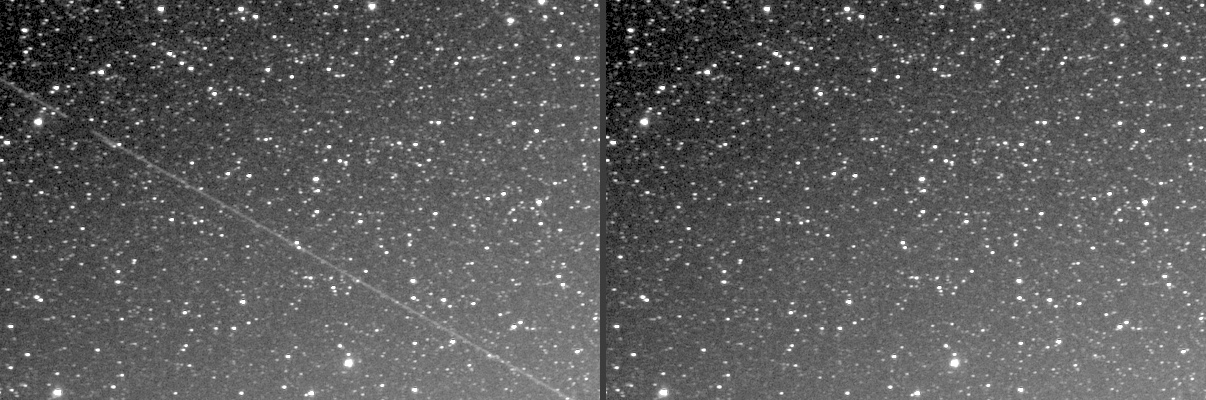
\includegraphics[width=0.9\linewidth]{figures/photo_sigma_trail}
\caption{シグマクリッピングの効果（左：ふつうの平均、右：シグマクリッピング）。人工衛星の光跡が消えます}
\end{figure}

\begin{caution}[流れる雲や明滅する灯り]
時間とともに変わるもの（流れる雲、明るさの変わる街の灯りなど）は、画素ごとに残る写真が変わるため、角張ったむらになることがあります。
気になるときは、シグマクリッピングを外してください。
\end{caution}

\begin{figure}[H]
\centering
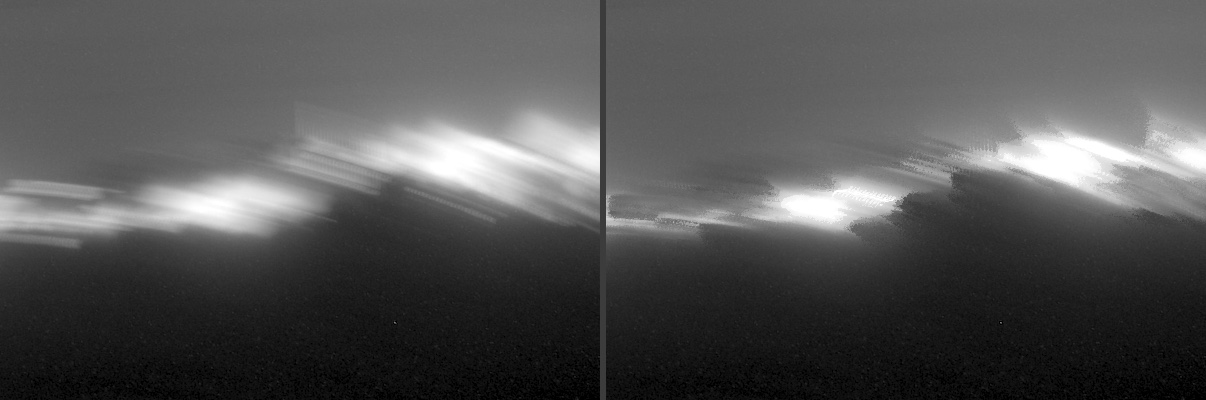
\includegraphics[width=0.9\linewidth]{figures/photo_sigma_cloud}
\caption{流れる雲と街の灯りの所（左：ふつうの平均、右：シグマクリッピング）。右では角張ったむらになっています}
\end{figure}

\clearpage
\section{新星景モード（星も地上もくっきり）}\label{sec:nightscape}

\subsection{しくみ}

星は時間とともに動き、地上は動きません（追尾撮影では反対に、星が止まって地上が動きます）。
そのため、星に合わせて重ねると地上がにじみ、地上に合わせて重ねると星がにじみます。

新星景モードでは、\textbf{空は星に合わせて}、\textbf{地上は地上に合わせて}それぞれ重ね、空と地上の境目でつなぎ合わせます。
空と地上の境目は、写真を見比べて自動で見つけます。違っている所は、ブラシで塗って直せます。

\begin{center}
\begin{tikzpicture}[font=\sffamily\small,
  box/.style={draw=black!40,rounded corners=3pt,minimum width=3.2cm,minimum height=1.0cm,align=center},
  arr/.style={-{Stealth[length=2.4mm]},accentdark,line width=1pt}]
  \node[box,fill=skyblue!12] (sky) at (0,0.8) {空は\textbf{星}に合わせて重ねる};
  \node[box,fill=groundgreen!12] (ground) at (0,-0.8) {地上は\textbf{地上}に合わせて重ねる};
  \node[box,fill=accent!12,minimum width=3.6cm] (mix) at (5.2,0) {境目でつなぐ\\（自動で判定＋ブラシで直す）};
  \node[box,fill=black!5,minimum width=2.4cm] (out) at (9.4,0) {星も地上も\\くっきりした1枚};
  \draw[arr] (sky.east) -- (mix.west); \draw[arr] (ground.east) -- (mix.west); \draw[arr] (mix) -- (out);
\end{tikzpicture}
\end{center}

\begin{memo}
新星景モードは、スタック方式が\ui{平均}か\ui{中央値}のときに使えます（中央値を選んだ場合も、外れ値を除いた平均で合成します）。
動く星や飛行機の光を除くために、シグマクリッピングの κ の設定を使います。
\end{memo}

\subsection{使い方の流れ}

\begin{center}
\begin{tikzpicture}[node distance=0.32cm,
  box/.style={draw=accentdark,fill=accent!12,rounded corners=3pt,minimum height=1.1cm,text width=2.3cm,
    align=center,font=\sffamily\small},
  arr/.style={-{Stealth[length=2.4mm]},accentdark,line width=1pt}]
  \node[box] (a) {\textbf{1} 新星景モードを\\ON にする};
  \node[box,right=of a] (b) {\textbf{2}\ui{解析開始}\\を押す};
  \node[box,right=of b] (c) {\textbf{3} 違う所を\\ブラシで直す};
  \node[box,right=of c] (d) {\textbf{4} スタッキング\\開始};
  \node[box,right=of d] (e) {\textbf{5} 結果を見て\\必要なら塗り直す};
  \draw[arr] (a) -- (b); \draw[arr] (b) -- (c); \draw[arr] (c) -- (d); \draw[arr] (d) -- (e);
  \draw[arr] (e.south) -- ++(0,-0.45) -| (c.south);
\end{tikzpicture}
\end{center}

\subsubsection*{手順1　新星景モードを ON にする}

Light の写真を読み込み、スタック方式を\ui{平均}にしてから、\ui{空と地上（新星景モード）}の欄の\ui{新星景モード}にチェックを入れます。

\begin{figure}[H]
\centering
\begin{screenshot}[0.5\linewidth]{settings_nightscape}
  \calloutleft{1}{check}
  \calloutleft{2}{register}
  \calloutleft{3}{analyze}
  \calloutleft{4}{brush}
  \calloutleft{5}{size}
  \calloutleft{6}{feather}
  \calloutleft{7}{clearmask}
\end{screenshot}
\caption{\ui{空と地上（新星景モード）}の欄}
\end{figure}

\begin{callouts}
\co{1} \ui{新星景モード}：チェックを入れると、空と地上を分けて合成します。その下に、いまの状態や次にすることが表示されます。
\co{2} \ui{地上固定フレーム登録…}：地上だけを撮った写真を登録します（\ref{sec:groundfixed}節）。\ui{解除}で外します。
\co{3} \ui{解析開始}：全部の写真を調べて、空と地上を自動で塗り分けます。
\co{4} \textbf{ブラシの種類}：\ui{空（青）}・\ui{地上（緑）}・\ui{消しゴム}を選びます。
\co{5} \textbf{ブラシの大きさ}（5〜150 px）。
\co{6} \textbf{境界ぼかし}（0〜300 px、最初は 0 px）：空と地上の境目をさらになじませます（\ref{sec:feather}節）。
\co{7} \ui{マスクをクリア}：塗った色（自動の判定も含む）をすべて消します（\key{⌘}\,\key{K}）。
\end{callouts}

\subsubsection*{手順2　\ui{解析開始}を押す}

\ui{解析開始}を押すと、全部の写真の位置を星と地上のそれぞれで合わせ、空と地上を自動で判定します。
写真の枚数や Mac によって、数分かかります（ボタンに進み具合が表示されます）。

終わると、基準画像の上に、空が\textcolor{skyblue}{\textbf{青}}、地上が\textcolor{groundgreen}{\textbf{緑}}で半透明に塗られます。

\begin{figure}[H]
\centering
\begin{screenshot}{main_analyzed}
  \calloutat{1}{0.40}{0.70}{90}{0.9}
  \calloutat{2}{0.45}{0.28}{-90}{0.9}
  \calloutright{3}{status}
\end{screenshot}
\caption{解析が終わったところ。\num{1}空（青）と\num{2}地上（緑）に塗り分けられ、\num{3}に結果が表示されます}
\end{figure}

\begin{memo}[境目は塗られていません]
空と地上の境目のすぐ近くは、わざと塗らずに残してあります。境目は、合成するときに写真の輪郭に沿って自動で決めます。
\end{memo}

\subsubsection*{手順3　違う所をブラシで直す}

自動の判定が違っている所があれば、ブラシで塗り直します。
\begin{steps}
  \item \ui{空（青）}か\ui{地上（緑）}を選びます。
  \item プレビューの上でドラッグして塗ります。塗った所は、自動の判定より優先されます。
  \item 塗りすぎた所は\ui{消しゴム}で消すと、自動の判定に戻ります。
\end{steps}

\begin{figure}[H]
\centering
\begin{minipage}[t]{0.49\linewidth}\centering
\begin{screenshot}{canvas_analyzed}
  \circleat{0.07}{0.44}{1.0}
\end{screenshot}\\[0.3ex]{\small 直す前：左端の空の一部が地上（緑）になっている（左下を拡大）}
\end{minipage}\hfill
\begin{minipage}[t]{0.49\linewidth}\centering
\begin{screenshot}{canvas_brushed}
  \circleat{0.07}{0.44}{1.0}
\end{screenshot}\\[0.3ex]{\small 直した後：空（青）のブラシで塗った}
\end{minipage}
\caption{ブラシで直す例}
\end{figure}

\begin{hint}[ブラシのこつ]
\begin{itemize}[itemsep=0.2ex,leftmargin=1.2em]
  \item 境目ぴったりに塗る必要はありません。少しはみ出して塗っても、はみ出した所は写真の輪郭に合わせて自動で直ります。
  \item 細かい所は、写真を拡大してから（ピンチ、または\key{⌘}＋スクロール）小さなブラシで塗ります。
  \item 拡大した写真を動かすときは、\key{space}キーか\key{option}キーを押しながらドラッグします。
\end{itemize}
\end{hint}

\subsubsection*{手順4　スタッキング開始}

\ui{★ スタッキング開始}を押します。手順2の解析の結果を使うので、位置合わせはやり直しません。

\begin{figure}[H]
\centering
\begin{screenshot}{main_result}
  \calloutabove{1}{toggle}
  \calloutright{2}{status}
\end{screenshot}
\caption{新星景モードで合成したところ}
\end{figure}

\begin{callouts}
\co{1} \ui{元画像を表示}：押すと元の写真とマスクの表示に戻り、ブラシで塗り直せます。
\co{2} 「新星景モード・…で合成」と表示されれば、空と地上を分けて合成できています。
\end{callouts}

\subsubsection*{手順5　結果を見て、必要なら塗り直す}

結果を拡大して、空と地上の境目を確かめます。気になる所があれば、\ui{元画像を表示}を押してブラシで塗り直し、もう一度\ui{★ スタッキング開始}を押します。
2回目からは解析をやり直さないので、早く終わります。

\begin{caution}[解析をやり直すとき]
Light の写真・基準画像・Dark などを変えたときは、前の解析の結果は使えません。もう一度\ui{解析開始}を押してください（ブラシで塗った所は残ります）。
\end{caution}

\subsection{地上固定フレーム}\label{sec:groundfixed}

星を追尾して撮ると、地上は写真ごとに流れてしまいます。そのようなとき、追尾を止めて地上だけを撮った写真（\textbf{地上固定フレーム}）があれば、地上はその写真を使い、その構図で合成できます。

\begin{steps}
  \item 新星景モードをONにして、\ui{地上固定フレーム登録…}を押し、地上を撮った写真を選びます（何枚でも）。
  \item ファイルリストの Light タブのいちばん上に\ui{地上固定フレーム}の欄ができ、登録した写真が並びます。
  \item \ui{解析開始}を押します。今度は地上固定フレームの上に、空と地上が塗り分けられます。
  \item あとはふつうの新星景モードと同じです（ブラシで直して、スタッキング開始）。
\end{steps}

\begin{figure}[H]
\centering
\begin{screenshot}{main_groundfixed}
  \calloutleft{1}{section}
  \calloutright{2}{register}
\end{screenshot}
\caption{地上固定フレームを登録して解析したところ。\num{1}登録した写真、\num{2}登録のボタン（枚数が表示されます）}
\end{figure}

\begin{itemize}[itemsep=0.4ex]
  \item \textbf{撮り方}：Light と同じ三脚・同じ位置で、追尾撮影の\textbf{直前か直後}に続けて撮ってください。前と後の両方の写真を混ぜると、地上が二重になります（写真どうしの位置合わせはしません）。
  \item \textbf{複数枚}：画素ごとの中央値で1枚にまとめます（2枚なら平均）。露出の違う写真（AEB など）でもかまいません。撮影情報（露出時間・ISO・F値）から、明るさを Light に揃えます。白飛びした所は使いません。
  \item \textbf{補正}：Dark は露出時間が違うので、地上固定フレームには使いません（Flat・Bias は使います）。
  \item \textbf{RAW}：Light が RAW のときは、同じカメラの RAW を登録してください。
  \item \textbf{マスク}：登録したり外したりすると、マスクの構図が変わるので、塗ったマスクは消えます。もう一度\ui{解析開始}を押してください。
\end{itemize}

\begin{figure}[H]
\centering
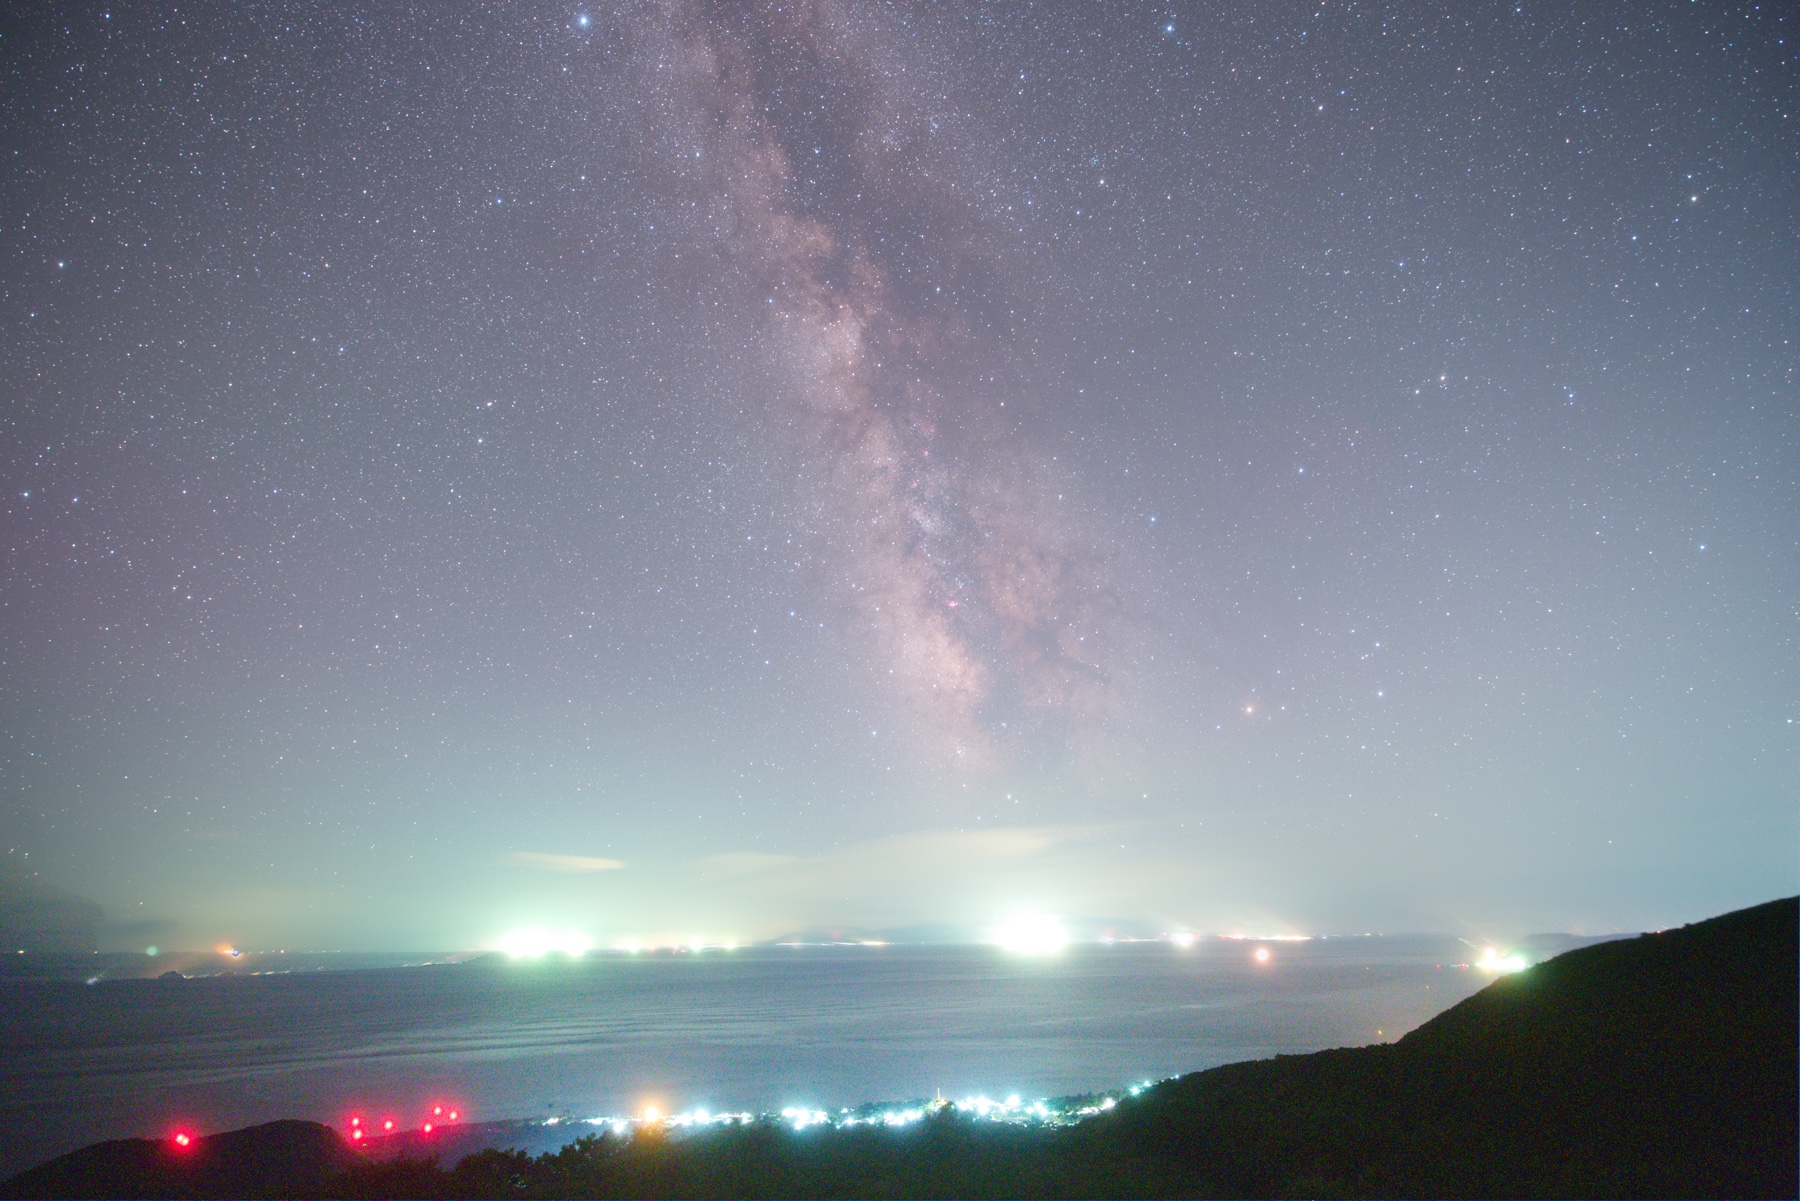
\includegraphics[width=\linewidth]{figures/photo_groundfixed}
\caption{地上固定フレーム（2枚、露出の違う AEB）を使って合成した例}
\end{figure}

\subsection{境界ぼかし}\label{sec:feather}

\ui{境界ぼかし}（0〜300 px）を大きくすると、空と地上の境目をなだらかにつなぎます。最初は 0 px（自動で決めた境目のまま）です。
\begin{itemize}[itemsep=0.3ex]
  \item 境目に線のような段差が見えるときに使います。100〜200 px くらいから試してください。
  \item 地上固定フレームを使うときは、地上の側にだけぼかします。空の星はそのままで、地上固定フレームのノイズや色味の違いを、境目の近くでなだらかにつなぎます。
  \item プレビューのマスクも、合成と同じだけぼかして表示されます。
\end{itemize}

\subsection{うまくいかないとき}

\begin{center}
\small
\begin{tabularx}{\linewidth}{>{\raggedright\arraybackslash}p{0.38\linewidth} X}
\toprule
表示・ようす & どうすればよいか \\
\midrule
「星と地上の動きの差が小さいため、空と地上を分けずに合成しました」 & 撮影時間が短く、星がほとんど動いていません。ふつうの合成で十分きれいになります。 \\
「空と地上をはっきり見分けられなかったため…」 & 空だけ・地上だけの構図です。ブラシで空と地上を塗ってから、もう一度\ui{解析開始}を押してみてください。 \\
空の一部が地上（または地上の一部が空）になる & ブラシで塗り直してから、スタッキング開始を押します。 \\
地上の明るい灯りのまわりが不自然 & 灯りのまわりを空（青）か地上（緑）で塗り分けると、改善することがあります。 \\
「…のメモリが必要なため実行できません」 & 写真の枚数を減らしてください。 \\
\bottomrule
\end{tabularx}
\end{center}

\clearpage
\section{比較明合成（星の軌跡）}\label{sec:startrail}

比較明合成では、画素ごとにいちばん明るい値を残すので、星が動いた跡が線（スタートレイル）になります。

\begin{figure}[H]
\centering
\begin{screenshot}[0.46\linewidth]{settings_comparebright}
  \calloutleft{1}{mode}
  \calloutleft{2}{align}
  \calloutleft{3}{trail}
  \calloutleft{4}{analyzetrails}
  \calloutleft{5}{mask}
\end{screenshot}
\caption{比較明合成を選んだところ}
\end{figure}

\begin{callouts}
\co{1} スタック方式で\ui{比較明合成 (Star Trails)}を選びます。
\co{2} \ui{アライメント}：最初は外れています。入れると星が点になります（ふつうは外したまま）。
\co{3} \ui{飛行機・人工衛星の光跡を除去}：チェックを入れると、合成の前に飛行機や人工衛星の光跡を探して取り除きます。
\co{4} \ui{光跡を解析して確認…}：光跡を探して、確認の画面を開きます（下）。
\co{5} \ui{空と地上を分けて合成（ブラシを使用）}：ブラシで塗った所を、空は比較明、地上は平均で合成します（下）。
\end{callouts}

\subsection{飛行機・人工衛星の光跡を取り除く}

\ui{飛行機・人工衛星の光跡を除去}にチェックを入れて\ui{★ スタッキング開始}（または\ui{光跡を解析して確認…}）を押すと、全部の写真から光跡を探し、確認の画面が開きます。

\begin{figure}[H]
\centering
\begin{screenshot}{trail_review}
  \calloutleft{1}{list}
  \calloutabove{2}{highlight}
  \calloutabove{3}{protect}
  \calloutabove{4}{all}
  \calloutbelow{5}{apply}
\end{screenshot}
\caption{光跡の確認の画面}
\end{figure}

\begin{callouts}
\co{1} 見つかった光跡の一覧です。\ui{除去}のチェックが入っているものを取り除きます。残したいもの（流れ星など）はチェックを外します。
\co{2} \ui{光跡ハイライトを表示}：見つかった光跡を色で示します。外すと元の写真を確かめられます。
\co{3} \ui{流星候補を保護}：流れ星らしいものを、取り除く対象から外します。
\co{4} \ui{全選択}・\ui{全解除}：全部のチェックを入れる・外します。
\co{5} \ui{確定してスタッキング開始}：チェックの入った光跡を取り除いて、合成を始めます。
\end{callouts}

光跡を取り除いた所は、前後の写真の同じ場所で埋めます。

\begin{memo}[星の軌跡を長くするには]
星の軌跡の長さは、撮影していた時間で決まります。三脚に固定して（星を追尾せずに）、長い時間続けて撮った写真を使ってください。
星を追尾して撮った写真では、星は止まったままで、地上が流れます。
\end{memo}

\subsection{空と地上を分けて合成する（比較明）}

比較明合成では、地上の部分もいちばん明るい値になるため、地上のノイズが目立つことがあります。
\ui{空と地上を分けて合成（ブラシを使用）}にチェックを入れ、プレビューで地上を\ui{地上（緑）}、空を\ui{空（青）}のブラシで塗ると、空は比較明、地上は平均で合成します。
\begin{itemize}[itemsep=0.3ex]
  \item 比較明合成では、空と地上の自動の判定は行いません。地上をブラシで塗ってください（塗らずにスタッキング開始を押すと、メッセージが出ます）。
  \item \ui{境界ぼかし}（0〜100 px、最初は 12 px）で、塗った境目をぼかします。
\end{itemize}

\clearpage
\section{結果を書き出す}\label{sec:export}

合成が終わったら、\ui{書き出し \& 実行}の欄で形式を選び、\ui{結果を書き出す…}（\key{⌘}\,\key{S}）を押します。
保存する場所と名前を決めるウインドウが開くので、\ui{保存}を押します。

\begin{center}
\small
\begin{tabularx}{\linewidth}{l X X}
\toprule
形式 & 中身 & こんなときに \\
\midrule
RAW (DNG) & RAW の写真だけを合成したときは、センサーのデータのまま（現像前）の DNG。そうでないときは 16bit のリニア DNG。 & Lightroom・Camera Raw などで、元の RAW と同じように露出・ホワイトバランス・ハイライトなどを調整したいとき（おすすめ）。 \\
16bit TIFF & 現像した 16bit のカラー画像。 & Photoshop などで仕上げるとき。 \\
32bit FITS & 32bit 浮動小数点のカラー画像（R・G・B の3面）。 & Siril・PixInsight などの天体画像処理ソフトで仕上げるとき。 \\
High Quality JPEG & 高画質の JPEG。 & そのまま SNS などで見せるとき。 \\
\bottomrule
\end{tabularx}
\end{center}

\begin{memo}[RAW のまま合成されるとき]
読み込んだ写真（Light・Dark・Flat・Bias）が、すべて同じカメラの RAW（ベイヤー配列）のときは、現像せずにセンサーのデータのまま合成します。
JPEG や TIFF が混ざっているとき、X-Trans などのセンサーのときは、現像した画像で合成します。
どちらで合成したかは、合成が終わったときのメッセージに表示されます。
\end{memo}

\begin{hint}[Lightroom で開いたとき]
RAW (DNG) は「Adobe 標準」のプロファイルで開きます。カメラの仕上がり設定（ピクチャースタイルなど）に近づけたいときは、プロファイルの一覧から選び直してください。
\end{hint}

\subsection{レンズプロファイル}

\begin{itemize}[itemsep=0.3ex]
  \item 基準画像の撮影情報から、カメラ・レンズ・焦点距離・F値・ISO・露出時間を表示します。
  \item \ui{DNGにレンズプロファイルを埋め込む}：チェックを入れると、DNG にレンズの情報を入れます。Lightroom などで開いたときに、レンズの補正（歪み・周辺減光）が自動で使われます。DNG で書き出すときだけ使われます。
  \item \ui{手動レンズ名}：撮影情報にレンズ名が入っていない（マニュアルレンズなど）ときは、ここにレンズ名を入れると DNG に書き込みます。
\end{itemize}

\clearpage
\section{タイムラプス動画を作る（設定の\ui{タイムラプス}タブ）}\label{sec:timelapse}

ファイルリストの Light の写真を順番につないで、動画（MP4）にします。設定の上のタブで\ui{タイムラプス}を選びます。

\begin{figure}[H]
\centering
\begin{screenshot}[0.46\linewidth]{settings_timelapse}
  \calloutright{1}{range}
  \calloutright{2}{speed}
  \calloutleft{3}{align}
  \calloutleft{4}{deflicker}
  \calloutleft{5}{autostretch}
  \calloutleft{6}{resolution}
  \calloutleft{7}{codec}
  \calloutleft{8}{write}
\end{screenshot}
\caption{設定の\ui{タイムラプス}タブ}
\end{figure}

\begin{callouts}
\co{1} \textbf{フレーム範囲}：動画に使う写真の範囲（開始フレーム・終了フレーム）を選びます。下に、使う枚数と、できる動画のおよその長さが表示されます。
\co{2} \textbf{再生速度}：\ui{FPS指定}（1秒に何枚の写真を見せるか、1〜120）か、\ui{秒数指定}（動画の長さ）を選び、数を入れて\key{return}キーで決めます。最初は 24 fps です。
\co{3} \textbf{位置合わせ}：\ui{位置合わせなし}・\ui{地上に合わせる（揺れ補正）}・\ui{星に合わせる（星を固定）}から選びます。
\co{4} \ui{フリッカー除去（輝度均一化）}：写真ごとの明るさのばらつき（ちらつき）をそろえます。
\co{5} \ui{オートストレッチ}：暗い写真を見やすい明るさにしてから動画にします。
\co{6} \textbf{解像度}：\ui{オリジナル}・\ui{4K}・\ui{1080p}・\ui{720p}から選びます。
\co{7} \textbf{コーデック}：\ui{H.264}か\ui{H.265/HEVC}を選びます。HEVC はファイルが小さくなりますが、古い機器では再生できないことがあります。
\co{8} \ui{タイムラプス書き出し}：保存する場所を選んで、動画を書き出します。
\end{callouts}

\begin{center}
\small
\begin{tabularx}{\linewidth}{l X}
\toprule
位置合わせ & こんなときに \\
\midrule
位置合わせなし & 三脚でしっかり固定して撮ったとき。 \\
地上に合わせる（揺れ補正） & 風で三脚がゆれた、追尾撮影で地上が動いたなど、地上を止めたいとき（星は動きます）。 \\
星に合わせる（星を固定） & 星空を止めて、地上が回っていくように見せたいとき。 \\
\bottomrule
\end{tabularx}
\end{center}

\begin{memo}[macOS10.13 版]
\textsf{macOS10.13} 版では、HEVC（H.265）は、HEVC のハードウェアエンコーダーがある Mac でだけ選べます。
\end{memo}

\clearpage
\section{設定項目の一覧}\label{sec:reference}

\small
\renewcommand{\arraystretch}{1.15}
\begin{tabularx}{\linewidth}{>{\raggedright\arraybackslash}p{0.27\linewidth} >{\raggedright\arraybackslash}p{0.17\linewidth} X}
\toprule
項目 & 最初の値 & 説明 \\
\midrule
\multicolumn{3}{l}{\textbf{スタック方式}} \\
スタック方式 & 平均 & 平均・中央値・比較明合成（\ref{sec:stacking}節）。 \\
アライメント & 平均・中央値：ON／比較明：OFF & 星の位置を合わせてから重ねます。新星景モードでは常に使います。 \\
シグマクリッピング & OFF & 平均のときだけ。外れ値を除いてから平均します。 \\
κ 下側・上側 & 3.0・3.0 & 1〜10。小さいほど多くの値を外れ値として除きます。新星景モードでも使います。 \\
光跡を除去 & OFF & 比較明合成のときだけ。飛行機・人工衛星の光跡を取り除きます。 \\
\midrule
\multicolumn{3}{l}{\textbf{空と地上（新星景モード）}} \\
新星景モード & OFF & 平均・中央値のとき。空と地上を分けて合成します。 \\
空と地上を分けて合成 & OFF & 比較明合成のとき。ブラシで塗った地上を平均で合成します。 \\
ブラシ & 空（青）、20 px & 空（青）・地上（緑）・消しゴム、大きさ 5〜150 px。 \\
境界ぼかし & 新星景：0 px／比較明：12 px & 新星景 0〜300 px、比較明 0〜100 px。 \\
地上固定フレーム & なし & 地上だけを撮った写真。地上はこの写真にします。 \\
\midrule
\multicolumn{3}{l}{\textbf{レンズプロファイル・書き出し}} \\
DNGにレンズプロファイルを埋め込む & ON & DNG で書き出すときにレンズの情報を入れます。 \\
手動レンズ名 & 空欄 & 撮影情報にレンズ名が無いときに入れます。 \\
書き出し形式 & RAW (DNG) & RAW (DNG)・16bit TIFF・32bit FITS・High Quality JPEG。 \\
\midrule
\multicolumn{3}{l}{\textbf{プレビュー}} \\
Auto Stretch & OFF & 表示だけを明るくします（結果は変わりません）。 \\
\midrule
\multicolumn{3}{l}{\textbf{タイムラプス}} \\
フレーム範囲 & 全部 & 動画に使う写真の範囲。 \\
再生速度 & 24 fps & FPS（1〜120）か、動画の秒数で指定。 \\
位置合わせ & 位置合わせなし & なし・地上に合わせる・星に合わせる。 \\
フリッカー除去 & OFF & 写真ごとの明るさをそろえます。 \\
オートストレッチ & OFF & 暗い写真を明るくしてから動画にします。 \\
解像度 & オリジナル & オリジナル・4K・1080p・720p。 \\
コーデック & H.264 & H.264・H.265/HEVC。 \\
\bottomrule
\end{tabularx}
\normalsize

\clearpage
\section{よくある質問・困ったとき}\label{sec:faq}

\newcommand\faq[2]{\paragraph{Q.\ #1}\mbox{}\\A.\ #2\par\medskip}

\faq{アプリが開けません（「開いていません」「開けません」と出る）。}{
MacStarStacker は Apple の Developer ID による署名・公証をしていないため、初めて開くときに止められます。
DMG の「かんたんインストーラ」を使うか、\ref{sec:install-manual}節の手順で開いてください。}

\faq{プレビューが真っ暗で、何が写っているか分かりません。}{
プレビューの上の\ui{Auto Stretch}にチェックを入れると、見やすい明るさで表示します（表示だけで、結果は変わりません）。}

\faq{合成した結果が暗い（または色が変）です。}{
RAW (DNG) で書き出した場合は、現像前のデータなので、Lightroom などで露出・ホワイトバランスを調整してください。元の RAW と同じように調整できます。}

\faq{「…のメモリが必要なため実行できません」と出ました。}{
中央値合成・シグマクリッピング・新星景モードは、全部の写真を一度にメモリに置きます。写真の枚数を減らすか、中央値の代わりに平均を使ってください。}

\faq{新星景モードで「空と地上を分けずに合成しました」と出ました。}{
メッセージに理由が表示されます。星がほとんど動いていない（撮影時間が短い）、空だけ・地上だけの構図、などです。\ref{sec:nightscape}節の「うまくいかないとき」を見てください。}

\faq{星の位置合わせに失敗しました、と出ます。}{
雲が多い、星が少ない（明るすぎる・ピントが合っていない）写真があると、位置を合わせられないことがあります。その写真をファイルリストから外して（\ui{×}）やり直してください。}

\faq{JPEG の写真でも使えますか？}{
使えます。ただし RAW で撮った写真の方が、合成した後に明るさや色を大きく調整しても画質が落ちにくいのでおすすめです。}

\faq{古い Mac（Metal に対応していない Mac）でも使えますか？}{
\textsf{macOS10.13} 版では、Metal（GPU）が使えない Mac では CPU で合成します。時間はかかりますが、結果は同じです。
また、RAW のプレビューは読み込みに時間がかかることがあります。}

\faq{作業を最初からやり直したいです。}{
ファイルリストの右上の\ui{すべてクリア}（または\menu{編集 → すべてクリア…}）で、起動した直後の状態に戻せます。}


\end{document}
